\documentclass[11pt,letterpaper]{article}
\usepackage{samstyle}

\title{
	Taller 1\\  
	Programación de Computadores\\
	Grupo 063
}

% \author{

% }

\begin{document}
 
\pagestyle{fancyplain}
\fancyhf{}
\headheight=20pt %para cambiar el tamaño del encabezado
\renewcommand{\headrulewidth}{0pt} %espesor del encabezado

% \lhead %la "L" indica a la izquierda
% {
% }

%\fancyfoot[c]{\thepage}

\maketitle

% \begin{minipage}{3cm}
% %\includegraphics[width=15cm]{aux/SamCanny.jpg}
% \end{minipage}

%

\section{CARACTERÍSTICAS: Suficientable}

En este curso se presenta una visión general de cómo programar un computador, incluyendo las relaciones que existen entre el programa y la máquina (el software y el hardware), los pasos en la creación de los programas y particularidades de diferentes lenguajes de programación.

El computador nos proporciona aquella información requerida por nosotros que quizás sin él sería inalcanzable, pero la máquina por sí sola no lo hace, por su cuenta no resuelve problemas comerciales, ni problemas científicos, ni de ningún tipo. Mientras no le suministremos una serie detallada de instrucciones para que nos resuelva esos problemas y nos brinde la información que buscamos, el computador es sencillamente una curiosidad de mucho valor que, en vez de ser útil, estorba.

\section{OBJETIVOS GENERALES DEL CURSO}

Al finalizar este curso, el estudiante:

\begin{itemize}
	\item Tendrá bases lógicas y técnicas para la programación de un computador 

	\item Poseerá conocimientos suficientes que le permitirán organizar y escribir instrucciones para un computador, es decir, programarlo de una manera eficaz mediante la utilización de un lenguaje de programación

	\item Erradicará la creencia que llevan algunas personas de que la programación es privilegio sólo de pocos, y así se sentirá bastante satisfecho de tener un computador a "sus órdenes"

	\item Comprenderá que no saber programar un computador, implica una merma, en un gran porcentaje, del producto del trabajo realizado con el mismo, a pesar del software tan desarrollado existente en el mercado
\end{itemize}

Texto Guia \cite{farrell2011programming}

\includegraphics[width=15cm]{SamCanny.jpg}


% \newpage

% \newpage
\begin{center}
\begin{tabular}{c c}
	Profesor & Monitor \\
	Sergio Andrés Monsalve Castañeda & Marcos David Sierra Gallego\\
	smonsal3@eafit.edu.co & msierr37@eafit.edu.co
\end{tabular}
\end{center}
\vspace{1cm} 

Para el primer taller de la semana es necesario que lleven resueltos los siguientes ejercicios de CodingBat\cite{Codingbat}, de los cuales les entregamos una rápida traducción.

\begin{enumerate}
	\item Python \textgreater Warmup-2 \textgreater front\_times:\\
		Dada una cadena y un entero no negativo (n), diremos que el frente de la cadena son los 3 primeros caracteres o lo que sea que haya en caso de que la longitud de la cadena sea menor a 3, retorne 3 copias del frente de la cadena. 

	\item Python \textgreater Warmup-1 \textgreater sum\_double:\\
		Dados dos números (a y b) retorne su suma, en caso de que a y b sean iguales retorne el doble de la suma de ambos.

	\item Python \textgreater String-2 \textgreater xyz\_there:\\
		Retorne verdadero si la cadena de caracteres dada contiene una aparición de \"xyz\", donde xyz no esta inmediatamente precedida de un punto (.) por lo que \"xxyz\" es valido pero \"x.xyz\" no.
	
	\item Python \textgreater String-1 \textgreater non\_start:\\
		Dadas 2 cadenas(a,b), retorne la concatenación de ambas (a+b), excepto el primer caracter de ambas, las cadenas tendrán longitud mayor o igual a 1.

	\item Python \textgreater String-1 \textgreater combo\_string:\\
		Dadas 2 cadenas (a,b) retorne una cadena de la forma corta+larga+corta, con la cadena corta en la parte de afuera de la cadena resultante y la larga adentro. Las cadenas nunca serán del mismo tamaño, mas pueden ser de longitud 0. 
\end{enumerate}


\bibliographystyle{IEEEtran}
\bibliography{Refs}

\end{document}